\documentclass{standalone}
\usepackage{xcolor}
\usepackage{tikz}
\usetikzlibrary{positioning, shapes.multipart, calc, graphs, graphs.standard}
\begin{document}
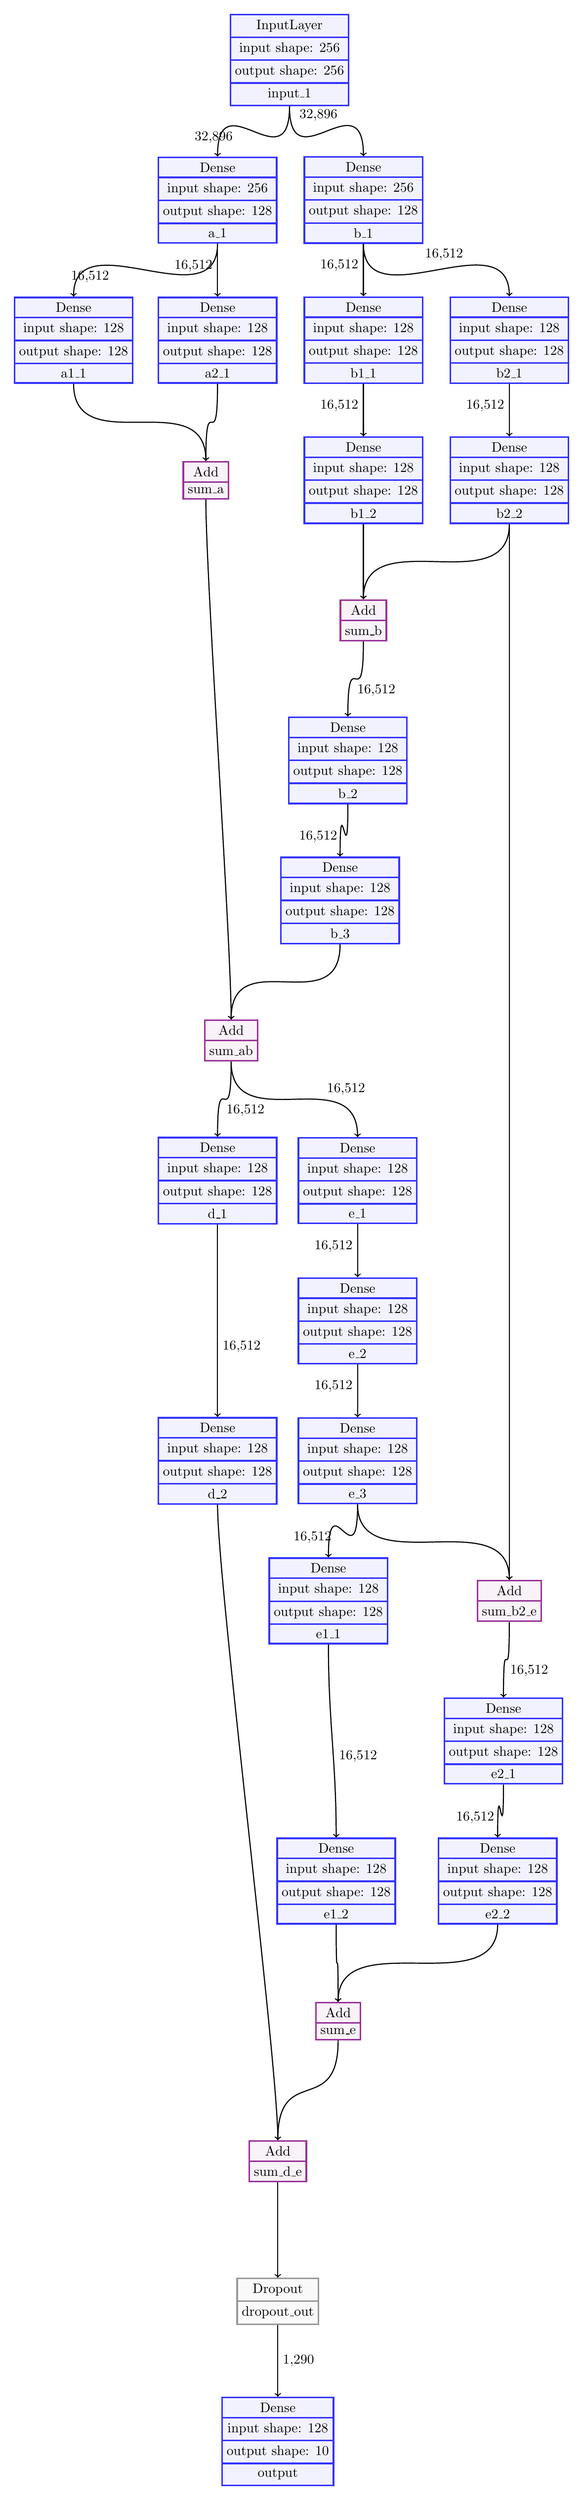
\begin{tikzpicture}
% style: default_edge
\tikzstyle{default_edge}=[thick,out=-90,in=90,out distance=2cm,in distance=2cm]
% style: default_label
\tikzstyle{default_label}=[auto,pos=0.65]
% style: TrainableLayer_style
\tikzstyle{TrainableLayer_style}=[rectangle split,rectangle split ignore empty parts,very thick,node distance=2cm,draw=blue!80,fill=blue!5]
% style: OperationLayer_style
\tikzstyle{OperationLayer_style}=[rectangle split,rectangle split ignore empty parts,very thick,node distance=1cm,draw=violet!80,fill=violet!5]
% style: UtilityLayer_style
\tikzstyle{UtilityLayer_style}=[rectangle split,rectangle split ignore empty parts,very thick,node distance=0cm,draw=gray!80,fill=gray!5]

% node: input_1
\node[TrainableLayer_style] (input_1) at (6.9475, 62.1)
    {
    \nodepart{one}{InputLayer}
    \nodepart{two}{input shape: 256}
    \nodepart{three}{output shape: 256}
    \nodepart{four}{input\_1}};

% node: b_1
\node[TrainableLayer_style] (b_1) at (8.8475, 58.5)
    {
    \nodepart{one}{Dense}
    \nodepart{two}{input shape: 256}
    \nodepart{three}{output shape: 128}
    \nodepart{four}{b\_1}};

% node: b1_1
\node[TrainableLayer_style] (b1_1) at (8.8475, 54.9)
    {
    \nodepart{one}{Dense}
    \nodepart{two}{input shape: 128}
    \nodepart{three}{output shape: 128}
    \nodepart{four}{b1\_1}};

% node: b2_1
\node[TrainableLayer_style] (b2_1) at (12.5975, 54.9)
    {
    \nodepart{one}{Dense}
    \nodepart{two}{input shape: 128}
    \nodepart{three}{output shape: 128}
    \nodepart{four}{b2\_1}};

% node: b1_2
\node[TrainableLayer_style] (b1_2) at (8.8475, 51.3)
    {
    \nodepart{one}{Dense}
    \nodepart{two}{input shape: 128}
    \nodepart{three}{output shape: 128}
    \nodepart{four}{b1\_2}};

% node: b2_2
\node[TrainableLayer_style] (b2_2) at (12.5975, 51.3)
    {
    \nodepart{one}{Dense}
    \nodepart{two}{input shape: 128}
    \nodepart{three}{output shape: 128}
    \nodepart{four}{b2\_2}};

% node: a_1
\node[TrainableLayer_style] (a_1) at (5.0975, 58.5)
    {
    \nodepart{one}{Dense}
    \nodepart{two}{input shape: 256}
    \nodepart{three}{output shape: 128}
    \nodepart{four}{a\_1}};

% node: sum_b
\node[OperationLayer_style] (sum_b) at (8.8475, 47.7)
    {
    \nodepart{one}{Add}
    \nodepart{two}{sum\_b}};

% node: a1_1
\node[TrainableLayer_style] (a1_1) at (1.3974, 54.9)
    {
    \nodepart{one}{Dense}
    \nodepart{two}{input shape: 128}
    \nodepart{three}{output shape: 128}
    \nodepart{four}{a1\_1}};

% node: a2_1
\node[TrainableLayer_style] (a2_1) at (5.0975, 54.9)
    {
    \nodepart{one}{Dense}
    \nodepart{two}{input shape: 128}
    \nodepart{three}{output shape: 128}
    \nodepart{four}{a2\_1}};

% node: b_2
\node[TrainableLayer_style] (b_2) at (8.4475, 44.1)
    {
    \nodepart{one}{Dense}
    \nodepart{two}{input shape: 128}
    \nodepart{three}{output shape: 128}
    \nodepart{four}{b\_2}};

% node: sum_a
\node[OperationLayer_style] (sum_a) at (4.7974, 51.3)
    {
    \nodepart{one}{Add}
    \nodepart{two}{sum\_a}};

% node: b_3
\node[TrainableLayer_style] (b_3) at (8.247499999999999, 40.5)
    {
    \nodepart{one}{Dense}
    \nodepart{two}{input shape: 128}
    \nodepart{three}{output shape: 128}
    \nodepart{four}{b\_3}};

% node: sum_ab
\node[OperationLayer_style] (sum_ab) at (5.4475, 36.9)
    {
    \nodepart{one}{Add}
    \nodepart{two}{sum\_ab}};

% node: e_1
\node[TrainableLayer_style] (e_1) at (8.6975, 33.3)
    {
    \nodepart{one}{Dense}
    \nodepart{two}{input shape: 128}
    \nodepart{three}{output shape: 128}
    \nodepart{four}{e\_1}};

% node: e_2
\node[TrainableLayer_style] (e_2) at (8.6975, 29.7)
    {
    \nodepart{one}{Dense}
    \nodepart{two}{input shape: 128}
    \nodepart{three}{output shape: 128}
    \nodepart{four}{e\_2}};

% node: e_3
\node[TrainableLayer_style] (e_3) at (8.6975, 26.1)
    {
    \nodepart{one}{Dense}
    \nodepart{two}{input shape: 128}
    \nodepart{three}{output shape: 128}
    \nodepart{four}{e\_3}};

% node: sum_b2_e
\node[OperationLayer_style] (sum_b2_e) at (12.5975, 22.5)
    {
    \nodepart{one}{Add}
    \nodepart{two}{sum\_b2\_e}};

% node: e1_1
\node[TrainableLayer_style] (e1_1) at (7.9475, 22.5)
    {
    \nodepart{one}{Dense}
    \nodepart{two}{input shape: 128}
    \nodepart{three}{output shape: 128}
    \nodepart{four}{e1\_1}};

% node: e2_1
\node[TrainableLayer_style] (e2_1) at (12.4475, 18.9)
    {
    \nodepart{one}{Dense}
    \nodepart{two}{input shape: 128}
    \nodepart{three}{output shape: 128}
    \nodepart{four}{e2\_1}};

% node: d_1
\node[TrainableLayer_style] (d_1) at (5.0975, 33.3)
    {
    \nodepart{one}{Dense}
    \nodepart{two}{input shape: 128}
    \nodepart{three}{output shape: 128}
    \nodepart{four}{d\_1}};

% node: e1_2
\node[TrainableLayer_style] (e1_2) at (8.147499999999999, 15.3)
    {
    \nodepart{one}{Dense}
    \nodepart{two}{input shape: 128}
    \nodepart{three}{output shape: 128}
    \nodepart{four}{e1\_2}};

% node: e2_2
\node[TrainableLayer_style] (e2_2) at (12.2975, 15.3)
    {
    \nodepart{one}{Dense}
    \nodepart{two}{input shape: 128}
    \nodepart{three}{output shape: 128}
    \nodepart{four}{e2\_2}};

% node: d_2
\node[TrainableLayer_style] (d_2) at (5.0975, 26.1)
    {
    \nodepart{one}{Dense}
    \nodepart{two}{input shape: 128}
    \nodepart{three}{output shape: 128}
    \nodepart{four}{d\_2}};

% node: sum_e
\node[OperationLayer_style] (sum_e) at (8.1975, 11.7)
    {
    \nodepart{one}{Add}
    \nodepart{two}{sum\_e}};

% node: sum_d_e
\node[OperationLayer_style] (sum_d_e) at (6.647499999999999, 8.1)
    {
    \nodepart{one}{Add}
    \nodepart{two}{sum\_d\_e}};

% node: dropout_out
\node[UtilityLayer_style] (dropout_out) at (6.647499999999999, 4.5)
    {
    \nodepart{one}{Dropout}
    \nodepart{two}{dropout\_out}};

% node: output
\node[TrainableLayer_style] (output) at (6.647499999999999, 0.9)
    {
    \nodepart{one}{Dense}
    \nodepart{two}{input shape: 128}
    \nodepart{three}{output shape: 10}
    \nodepart{four}{output}};

% edge from input_1 to b_1
\draw[->, default_edge] (input_1) to node [default_label] {32,896} (b_1);

% edge from b_1 to b1_1
\draw[->, default_edge] (b_1) to node [default_label] {16,512} (b1_1);

% edge from b_1 to b2_1
\draw[->, default_edge] (b_1) to node [default_label] {16,512} (b2_1);

% edge from b1_1 to b1_2
\draw[->, default_edge] (b1_1) to node [default_label] {16,512} (b1_2);

% edge from b2_1 to b2_2
\draw[->, default_edge] (b2_1) to node [default_label] {16,512} (b2_2);

% edge from input_1 to a_1
\draw[->, default_edge] (input_1) to node [default_label] {32,896} (a_1);

% edge from b1_2 to sum_b
\draw[->, default_edge] (b1_2) to node [default_label] {} (sum_b);

% edge from b2_2 to sum_b
\draw[->, default_edge] (b2_2) to node [default_label] {} (sum_b);

% edge from a_1 to a1_1
\draw[->, default_edge] (a_1) to node [default_label] {16,512} (a1_1);

% edge from a_1 to a2_1
\draw[->, default_edge] (a_1) to node [default_label] {16,512} (a2_1);

% edge from sum_b to b_2
\draw[->, default_edge] (sum_b) to node [default_label] {16,512} (b_2);

% edge from a1_1 to sum_a
\draw[->, default_edge] (a1_1) to node [default_label] {} (sum_a);

% edge from a2_1 to sum_a
\draw[->, default_edge] (a2_1) to node [default_label] {} (sum_a);

% edge from b_2 to b_3
\draw[->, default_edge] (b_2) to node [default_label] {16,512} (b_3);

% edge from sum_a to sum_ab
\draw[->, default_edge] (sum_a) to node [default_label] {} (sum_ab);

% edge from b_3 to sum_ab
\draw[->, default_edge] (b_3) to node [default_label] {} (sum_ab);

% edge from sum_ab to e_1
\draw[->, default_edge] (sum_ab) to node [default_label] {16,512} (e_1);

% edge from e_1 to e_2
\draw[->, default_edge] (e_1) to node [default_label] {16,512} (e_2);

% edge from e_2 to e_3
\draw[->, default_edge] (e_2) to node [default_label] {16,512} (e_3);

% edge from e_3 to sum_b2_e
\draw[->, default_edge] (e_3) to node [default_label] {} (sum_b2_e);

% edge from b2_2 to sum_b2_e
\draw[->, default_edge] (b2_2) to node [default_label] {} (sum_b2_e);

% edge from e_3 to e1_1
\draw[->, default_edge] (e_3) to node [default_label] {16,512} (e1_1);

% edge from sum_b2_e to e2_1
\draw[->, default_edge] (sum_b2_e) to node [default_label] {16,512} (e2_1);

% edge from sum_ab to d_1
\draw[->, default_edge] (sum_ab) to node [default_label] {16,512} (d_1);

% edge from e1_1 to e1_2
\draw[->, default_edge] (e1_1) to node [default_label] {16,512} (e1_2);

% edge from e2_1 to e2_2
\draw[->, default_edge] (e2_1) to node [default_label] {16,512} (e2_2);

% edge from d_1 to d_2
\draw[->, default_edge] (d_1) to node [default_label] {16,512} (d_2);

% edge from e1_2 to sum_e
\draw[->, default_edge] (e1_2) to node [default_label] {} (sum_e);

% edge from e2_2 to sum_e
\draw[->, default_edge] (e2_2) to node [default_label] {} (sum_e);

% edge from d_2 to sum_d_e
\draw[->, default_edge] (d_2) to node [default_label] {} (sum_d_e);

% edge from sum_e to sum_d_e
\draw[->, default_edge] (sum_e) to node [default_label] {} (sum_d_e);

% edge from sum_d_e to dropout_out
\draw[->, default_edge] (sum_d_e) to node [default_label] {} (dropout_out);

% edge from dropout_out to output
\draw[->, default_edge] (dropout_out) to node [default_label] {1,290} (output);

\end{tikzpicture}\end{document}